\documentclass[a4paper,11pt]{article}
\usepackage[T1]{fontenc}
\usepackage[utf8]{inputenc}
\usepackage{lmodern}
\usepackage[francais]{babel}
\usepackage{fullpage}
\usepackage[colorlinks=true,linkcolor=black,urlcolor=black]{hyperref}
\usepackage{graphicx}
\usepackage{color}
\usepackage{pdfpages}
\usepackage{moreverb}

\title{Docmentation du module Alpiroc}
\author{Maxime Jay-Allemand}
\begin{document}

\maketitle
%\tableofcontents

\section{Description générale du module}
Le module Alpiroc apporte des nouvelles fonctionnalités au logiciel de gestion d'entreprise Dolibarr. Ce module propose une nouvelle présentation des documents "propositions commerciales", "commandes" et "factures". Cette nouvelle présentation est construite sur la base du modèle Azur présent par défaut. Le module est paramétrable et vous permet de modifier le contenu de ces documents. Ce module s'adresse en particulier aux artisans qui sont amenés à décrire de manière détaillée des travaux prévus. Voici les différentes fonctionnalités du module :\\
 \begin{itemize}
    \item La création de profils personnalisés dont le choix est possible lors de la rédaction des propositions commerciales et des factures.
    \item Le choix entre deux entêtes différentes : la classique "azur" et celle du module "alpiroc"
    \item L'écriture de titre dans ces documents (pour clairement séparer les tâches à réaliser).
    \item L'affichage des sous totaux par rubrique (entre deux titres insérés).
    \item Le choix des colonnes à afficher dans le tableau listant les produits ou service vendu.
    \item La gestion d'acompte à verser à la commande.
    \item Afficher ou non certaines parties des documents (les conditions de règlement, la note public, une phrase de remerciement, une zone de signature, la note privée de l'entreprise...).
    \item L'affichage d'une banderole brouillon.
    \item La création d'une lettre de rappel à partir d'une facture ou d'une proposition commerciale impayée.
  \end{itemize}
\section{Licence}
This program is free software; you can redistribute it and/or modify it under the terms of the GNU General Public License as published by the Free Software Foundation; either version 3 of the License, or (at your option) any later version.\\
This program is distributed in the hope that it will be useful, but WITHOUT ANY WARRANTY; without even the implied warranty of MERCHANTABILITY or FITNESS FOR A PARTICULAR PURPOSE.  See the GNU General Public License for more details.\\
You should have received a copy of the GNU General Public License along with this program. If not, see \href{http://www.gnu.org/licenses/}{http://www.gnu.org/licenses/}.
\section{Installation}
Ce module est compatible avec les versions de Dolibarr suivantes :
\begin{itemize}
  \item 3.5.3
  \item 3.5.4
  \item 3.5.5
  \item 3.6.0
  \item 3.6.1
  \item 3.7.0
  \item 3.7.1
  \item 3.8.0
  \item 3.8.2
\end{itemize}
Voici les étapes permettant d'installer ce module :
\begin{enumerate}
  \item Télécharger le dossier Alpiroc.zip et décompresser le
  \item Copier ce dossier dans le répertoire htdocs/ présent à la racine de l'installation du logiciel Dolibarr (cela dépend de la configuration de votre serveur, /var/www/html/ par défaut sous Debian ou dérivée).
  \item Assurez vous que les permissions du répertoire Alpiroc ainsi que ses fichiers inclus soit suffisante pour que votre serveur puissent y accéder.
  \item Aller dans Dolibarr, configuration, modules et activer le module Aliproc qui se trouve dans la rubrique "Autre". Cliquez que l’icône de configuration pour pouvoir accéder aux options.
\end{enumerate}

\subsection{Mise à jour}
Les mise à jour entre les différentes version du module ne sont pas supportée techniquement (écraser l'ancien répertoire sans avoir désactivé le module dans Dolibarr peux conduire à des bugs). Pour mettre à jour son module il faut procédé comme suit :\\

\begin{itemize}
   \item Désactivation du module dans Dolibarr
   \item Suppression du répertoire Alpiroc
   \item Ré-installation du module
 \end{itemize} 

\section{Utilisation du module}

\subsection{Configuration du module : création des "profils"}
Allez sur la page de configuration du module Alpiroc. Cette page est accessible depuis le menu configuration puis modules. Sur cette page, il vous est proposez de créer ou de modifier des profils existant. Commencez par ajouter un nouveau profil et configurez le avec les options proposés (pensez à valider à chaque fois (cliquer sur le boutton "modifier")).\\
Voici la liste des options :
\paragraph{Créer une factures, commandes ou propositions commerciales}
\begin{description}
  \item[Phrase de remerciement en bas de page :] Cette phrase est personnalisable dans la page de configuration du module. Pour qu'elle s'affiche, cette option doit être activée.
  \item[La note public :] La note public est une note que vous pouvez inclure dans vos propositions commerciales et factures via l'onglet Notes. Afin de personnalisé et d'automatiser l'affichage de cette note public, vous pouvez configurer un titre qui sera affiché toujours au-dessus de cette note.
  \item[La note privé :] La note public est une note que vous pouvez inclure dans vos propositions commerciales et factures via l'onglet Notes.
  \item[Contact :] Lors de la rédaction de vos propositions commerciales et factures, vous pouvez attribuer un ou plusieurs contacts via l'onglet Contacts/Adresses. Vous pouvez alors personnaliser un titre pour cette rubrique dans la page de configuration du module.
  \item[Les acomptes :]En activant cette option, un notification d'un acompte à versé à la commande s'affichera sur la proposition commerciale. La valeur de cette acompte est personnalisable dans la page de configuration du module (option toujours désactivé pour les factures et commandes).
  \item[Zone de signature :] Cette option permet de faire apparaître une zone de signature en bas à droite de la proposition commerciale (option toujours désactivé pour les factures et commandes).
  \item[La note privée de l'entreprise :] Cette note se configure dans la page de configuration de l'entreprise. Cette note s'affiche sous l'adresse de votre entreprise.
  \item[Colonne prix unitaire et quantité :] Selon les produits ou services vendus, il est parfois nécessaire d'afficher ou non ces colonnes. L'affichage est, par exemple, intéressant lorsque le client bénéficie d'une remise sur un article ou une prestation, car elles permettent de visualiser le coût initiale.
  \item[Colonne TVA :] Cette option permet de cacher la colonne mentionnant la TVA dans le tableau qui liste les produits et services. 
  \item[Les titres :] Des titres entre les articles ou prestations peuvent être affiché dans le tableau principale. Ces titres permettent de créer des rubriques contenant divers articles ou prestation. Ces rubriques seront utilisées pour afficher les sous-totaux. \textbf{L'insertion d'un titre s'opère lors de la saisie d'un produit ou d'un service (petite zone de texte située en dessous de la saisie d'un article). Ce titre sera alors affiché dans le document final juste au dessus de ce produit ou service.}
  \item[Sous-totaux :] Les sous-totaux sont dépendant de l'insertion de titre dans vos documents. Lors de l'activation de cette option, les titres sont considéré comme des rubriques et les sous-totaux sont calculés et affichés à la fin de chaque rubrique.
  \item[Affichage de l'entête : ] Cette option vous permet de cacher l'entête des documents sur les documents sui possèdent multiple page. L'entête ne sera affiché que sur la première page.
  \item[Affichage de la mention Mme,Mr :] Cette mention sera affiché devant le nom de l'individu si celui ci est enregistré comme un particulier.
\end{description}

\paragraph{Créer une lettre de rappel à partir d'une facture, proposition commerciale ou commande}
\begin{description}
  \item[Activation :] Lorsque l'option "Affiche seulement les totaux avec une phrase de description afin de créer une lettre de rappel" est activé, le tableau principale qui liste les articles est remplacé par un petit tableau qui rappel le montant total dû.
  \item[Personnalisation :] Un texte personnalisé peut-être affiché avant et après ce tableau. Personnalisez votre texte !
\end{description}

\subsection{Créer sa proposition commerciale avec le profil désiré}
Créer maintenant une nouvelle proposition commerciale. Sur la page de création, un nouveau menu déroulant apparaît : "choix du profil Alpiroc". Dans ce menu, choisissez parmi les profils que vous avez configuré. Ensuite dans la liste déroulante "modèle de document", choisissez "Alpiroc". Générer votre document ! A tout moment vous pouvez choisir un autre profil et générer de nouveau le même document. De plus vous pouvez toujours modifiez un profil existant depuis l'interface de configuration.


\section{Exemples - Captures d'écran}
Les figures suivantes vous permettent de comprendre un peu mieux comment configurer puis utiliser ce module selon vos besoins :

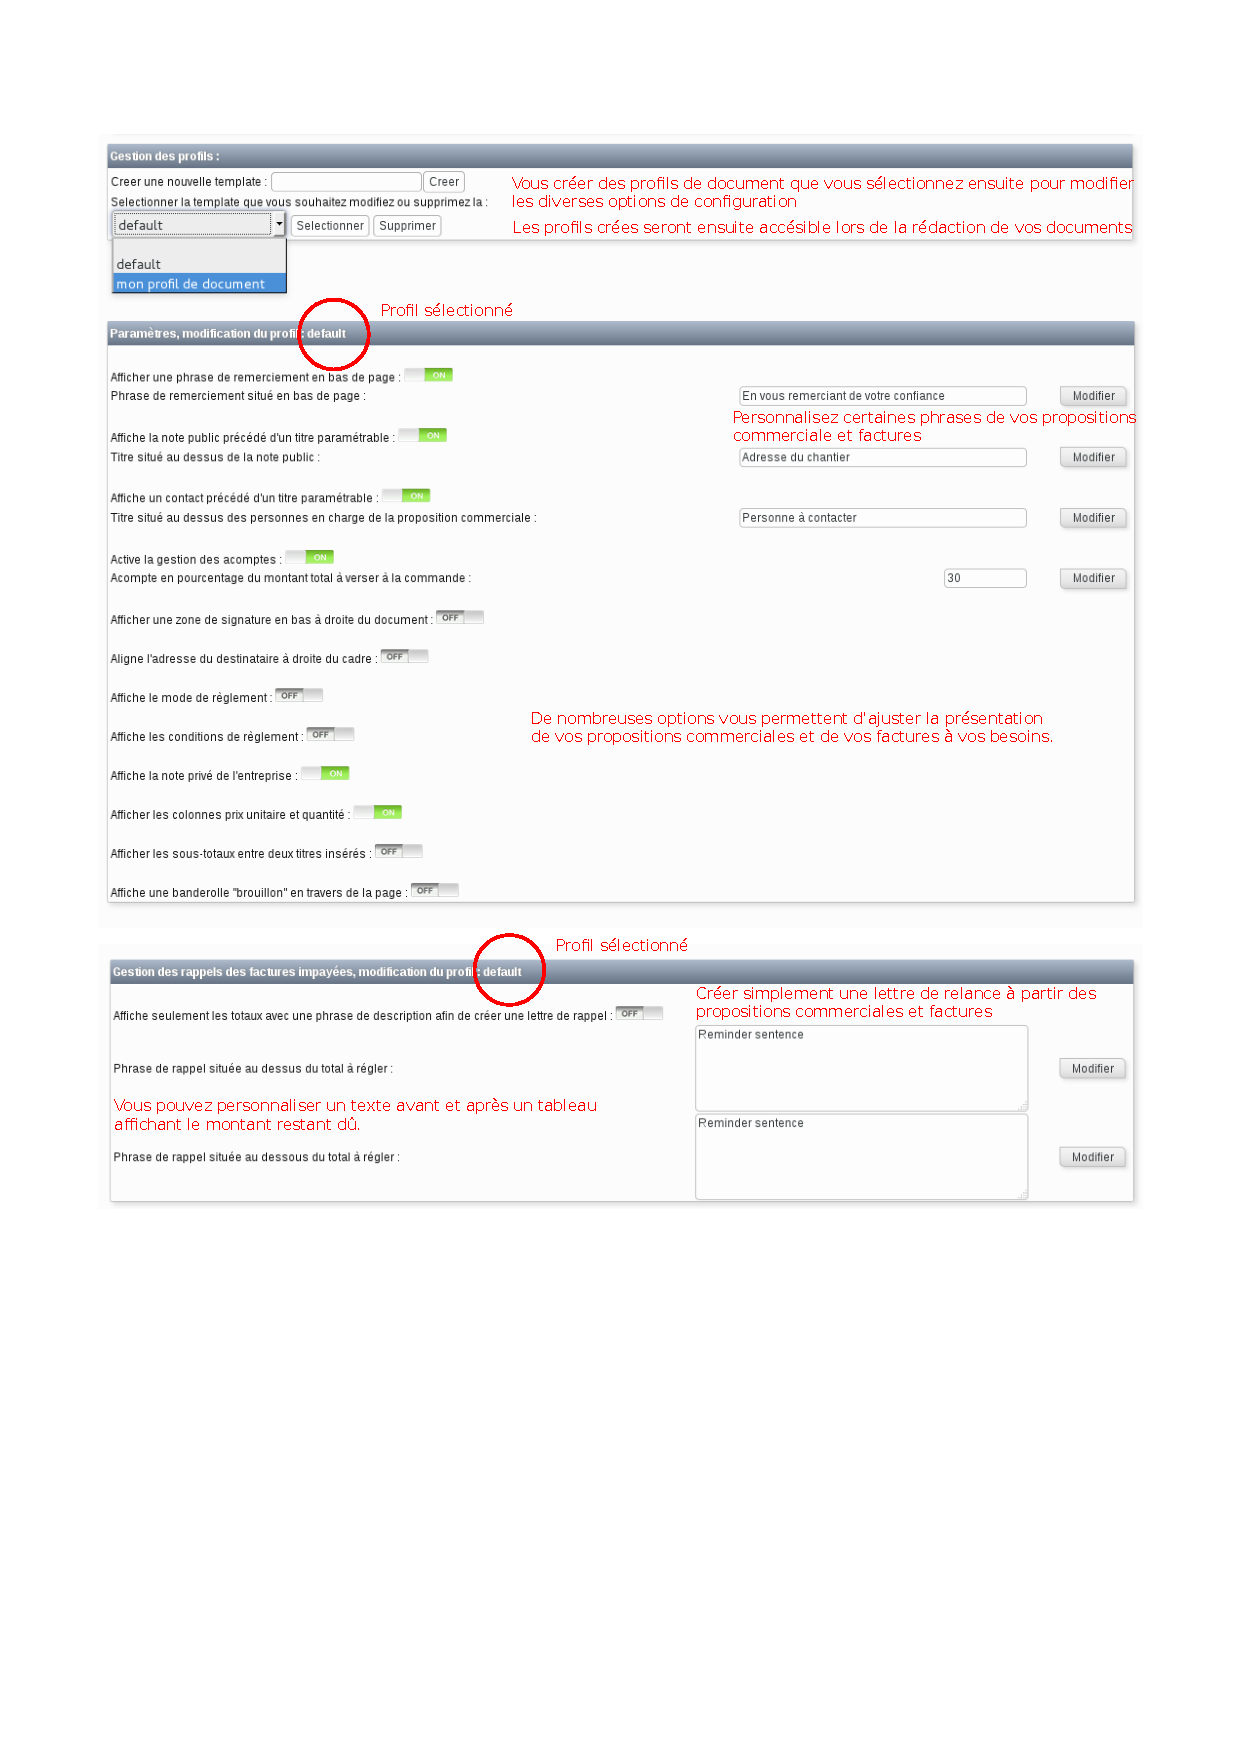
\includepdf[pages=-,pagecommand=\thispagestyle{plain}]{Configuration_annote.pdf}

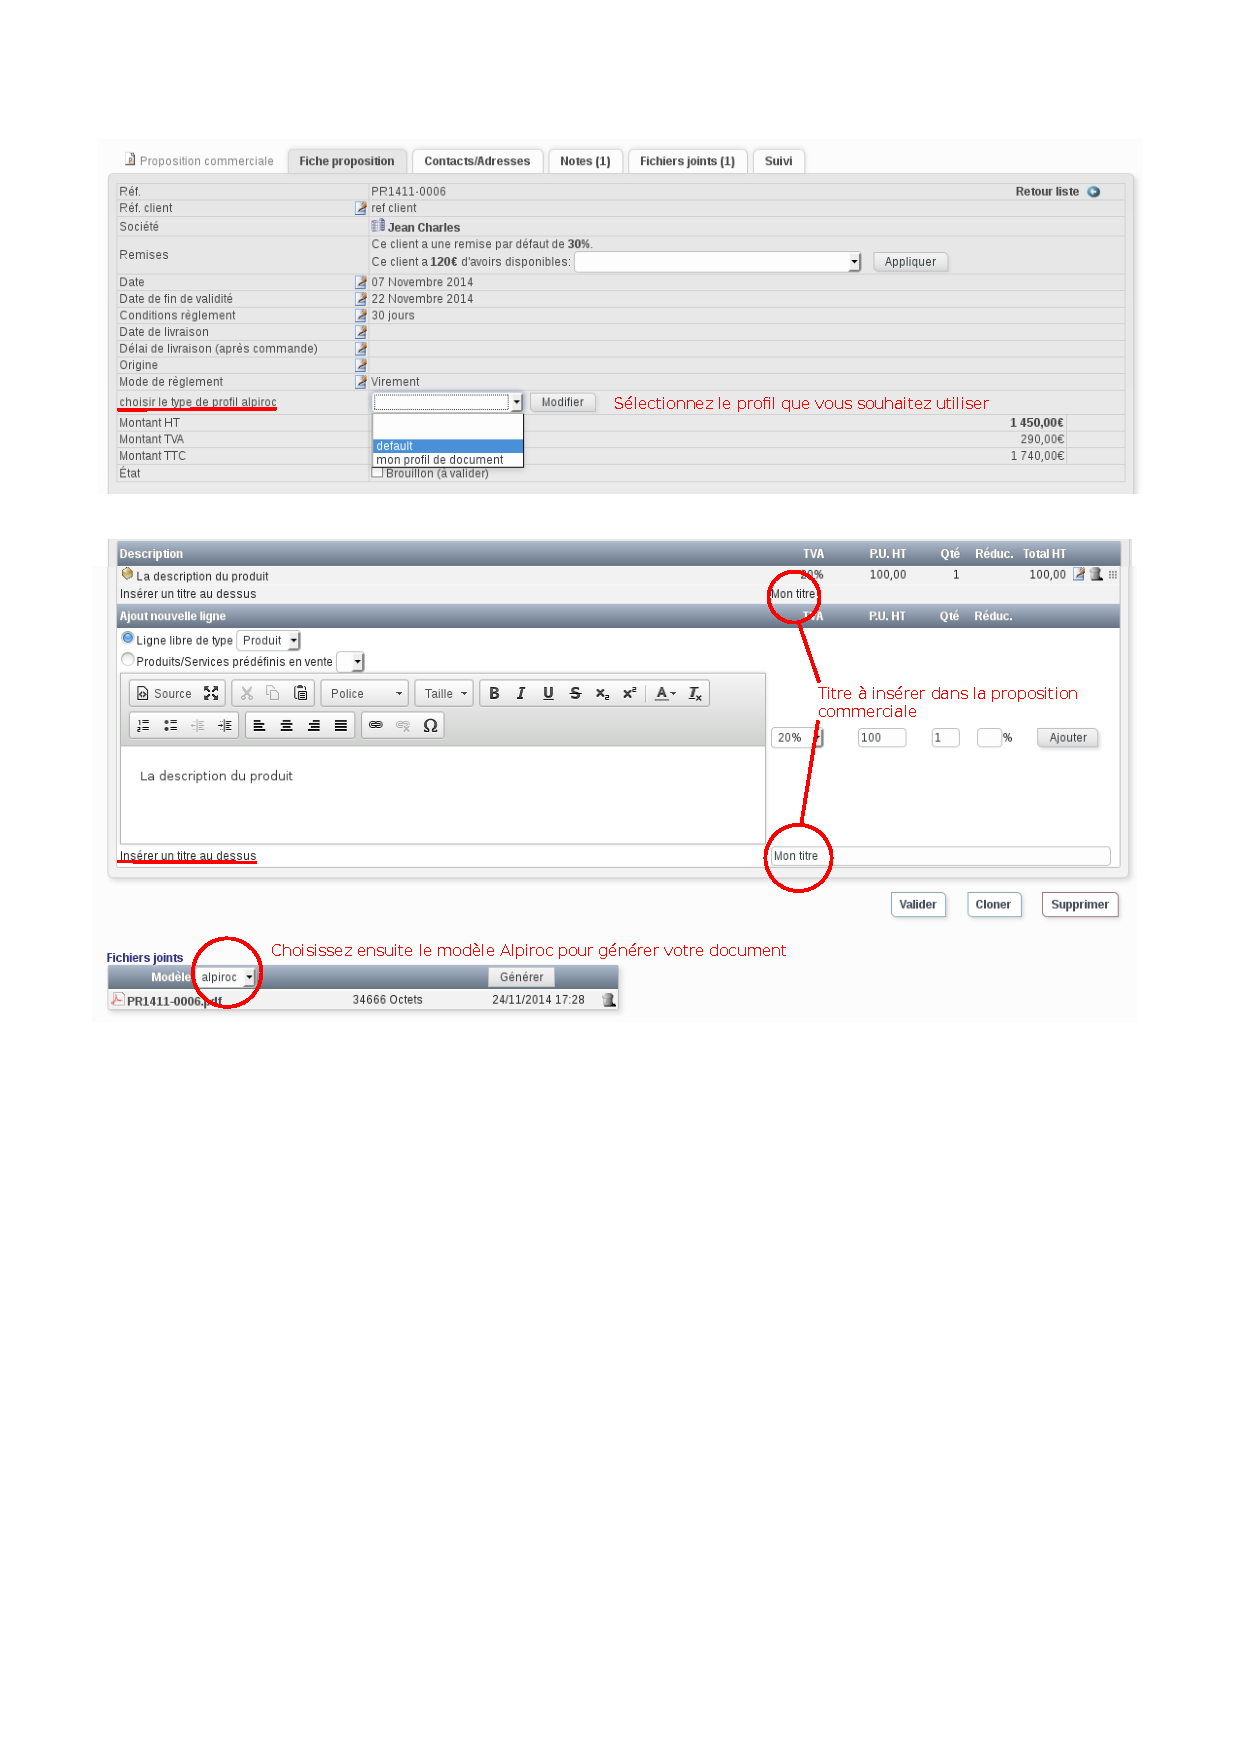
\includepdf[pages=-,pagecommand=\thispagestyle{plain}]{Redaction_annotations.pdf}


\section{Bidouilles, trucs et astuces}

\textit{\textbf{Avant de Bidouiller, sauvegarder toujours la version d'origine du fichier :)}}\\

\subsection{Personnaliser le texte :}
La plupart des textes dans les propositions commerciales sont stocké dans des fichiers situé dans le répertoire du module : Alpiroc$\slash$langs$\slash$fr\_FR (pour le francais). Vous pouvez allez modifiier les traductions en respectant bien le format du fichier : \\
\begin{center}
\textit{clé\_a\_ne\_pas\_modifié=mots\_modifiables}
\end{center}

\subsection{Génération des documents}
Le code permettant de généré les documents :\\
\begin{itemize}
  \item Proposition commerciale : $\slash$alpiroc$\slash$core modules$\slash$propale$\slash$doc$\slash$pdf\_alpiroc.modules.php
  \item Facture :$\slash$alpiroc$\slash$core $\slash$modules$\slash$facture$\slash$doc$\slash$core pdf\_alpiroc\_fact.modules.php
  \item Commande :$\slash$alpiroc$\slash$ core$\slash$modules$\slash$commande$\slash$doc$\slash$pdf\_alpiroc\_com.modules.php
\end{itemize}

\paragraph{Bidouille 1:\\}

Par exemple entre les lignes 220 et 270, les options du profil choisis sont chargés. 
\begin{verbatim}
 
			$alpiroc=new Alpiroc($this->db);

			$alpiroc->fetchValueFromProfil("dispreglement",$this->profil);
			$this->option_modereg=$alpiroc->content;//Affiche mode reglement
		
			$alpiroc->fetchValueFromProfil("dispcondreglement",$this->profil);
			$this->option_condreg=$alpiroc->content;//Affiche les conditions de reglement
		
			$alpiroc->fetchValueFromProfil("thanksarea",$this->profil);
			$this->option_conclusion_sentence=$alpiroc->content;//Phrase de conclusion en fin de page
		
			$alpiroc->fetchValueFromProfil("signaturearea",$this->profil);
			$this->option_sign_aera=$alpiroc->content;//Box de signature en bas à droite
		
			$alpiroc->fetchValueFromProfil("displayacompte",$this->profil);
			$this->option_acompte=$alpiroc->content;//Gestion des acomptes
			
			$alpiroc->fetchValueFromProfil("posadresse",$this->profil);
			$this->option_posaddresse=$alpiroc->content;	//Gestion des acomptes
		
			$alpiroc->fetchValueFromProfil("dispslogan",$this->profil);
			$this->option_slogan=$alpiroc->content;	//Gestion des acomptes
		
			$alpiroc->fetchValueFromProfil("displaypuqtx",$this->profil);//Gestion des colonne PU et QTX
			$this->option_prixunit_qty=$alpiroc->content;
			
			$alpiroc->fetchValueFromProfil("disptva",$this->profil);//Affichage de la colonne TVA
			$this->option_disp_tva=$alpiroc->content;//Affichage de la TVA
		
			$alpiroc->fetchValueFromProfil("soustotaux",$this->profil);
			$this->option_soustotaux=$alpiroc->content;	   //Affiche mode reglement
		
			$alpiroc->fetchValueFromProfil("brouillon",$this->profil);
			$this->option_brouillon=$alpiroc->content;	   //Affiche Brouillon
			
			$alpiroc->fetchValueFromProfil("rappel",$this->profil);
			$this->option_rappel=$alpiroc->content;	   //Affiche rappel
			
			$alpiroc->fetchValueFromProfil("notepublic",$this->profil);
			$this->option_notepublic=$alpiroc->content;	   //Affiche notepublic
			
			$alpiroc->fetchValueFromProfil("contact",$this->profil);
			$this->option_contact=$alpiroc->content;	   //Affiche contact
			
			$alpiroc->fetchValueFromProfil("repeathead",$this->profil);
			$this->option_repeat_head=$alpiroc->content;	   //Affiche contact

			$alpiroc->fetchValueFromProfil("hidedetails",$this->profil);
			$this->option_hidedetails=$alpiroc->content;	   //Affiche contact
			
			$alpiroc->fetchValueFromProfil("head",$this->profil);
			$this->option_head=$alpiroc->content;	   //choix de l'entête
			
			$alpiroc->fetchValueFromProfil("dispprivatenote",$this->profil);
			$this->option_dispprivatenote=$alpiroc->content;//Affichage de la note privé
			
			$alpiroc->fetchValueFromProfil("affichemmemr",$this->profil);
			$this->option_affichemmemr=$alpiroc->content;//Affichage Mme,Mr devant le nom
			
\end{verbatim}
Si pour vous souhaitez forcez une option à toujours être à la même valeur, il suffit d'ajouter une ligne comme dans l'exemple ci-après :
\begin{verbatim}
  $alpiroc->fetchValueFromProfil("affichemmemr",$this->profil);
	$this->option_affichemmemr=$alpiroc->content;//Affichage Mme,Mr devant le nom
  $this->option_affichemmemr=1; //LIGNE AJOUTEE
\end{verbatim}

Cette option égale à 1 sera désormais toujours activés dans votre document même si l'option est décoché dans la page de configuration.\\
Les options sont les suivantes  : 1 ou 0
\begin{itemize}
  \item 1 = Vrai = option activé
  \item 0 = Faux = option désactivé
\end{itemize}

Cela peut être utile si par exemple, pour les mêmes profils, vous souhaitez que les factures se comportent différemment. D'ailleurs par défaut, la zone de signature ne s'affichera jamais sur les factures. Si vous souhaitez modifier ce comportement, éditer le fichier qui génère le document facture et supprimé la ligne :
\begin{verbatim}
  $this->option_sign_aera=1;
\end{verbatim}

\paragraph{Bidouille 2:\\}

Juste après, entre les lignes 282 et 300, ce sont les options qui sont chargés si aucun profil n'est choisi (oubli par exemple) lors de la fabrication du pdf. Vous pouvez donc fabriquez votre profil par défaut personnalisé. Metez 1 ou 0 après le =, ou vous le souhaitez !

\begin{verbatim}
  			//Default value
			$this->option_modereg=1;
			$this->option_condreg=1;
			$this->option_conclusion_sentence=1;
			$this->option_sign_aera=1;
			$this->option_acompte=1;
			$this->option_slogan=1;
			$this->option_prixunit_qty=1;
			$this->option_disp_tva=1;
			$this->option_posaddresse=1;
			$this->option_soustotaux=0;
			$this->option_brouillon=0;
			$this->option_rappel=0;
			$this->option_contact=1;
			$this->option_notepublic=1;
			$this->option_repeat_head=1;
			$this->option_hidedetails=0;
			$this->option_head="alpiroc";
			$this->option_dispprivatenote=0;
			$this->option_affichemmemr=0;
\end{verbatim}


\section{Développement}
Le développement du module se fait via le débit sur Github à l'adresse suivante \url{https://github.com/maximejay/dolibarr\_alpiroc}.
La version en cours de développement est la branche master. Les autres branches sont les versions stables proposés sur le dolistore.



%\begin{figure}
% \begin{center}
 % 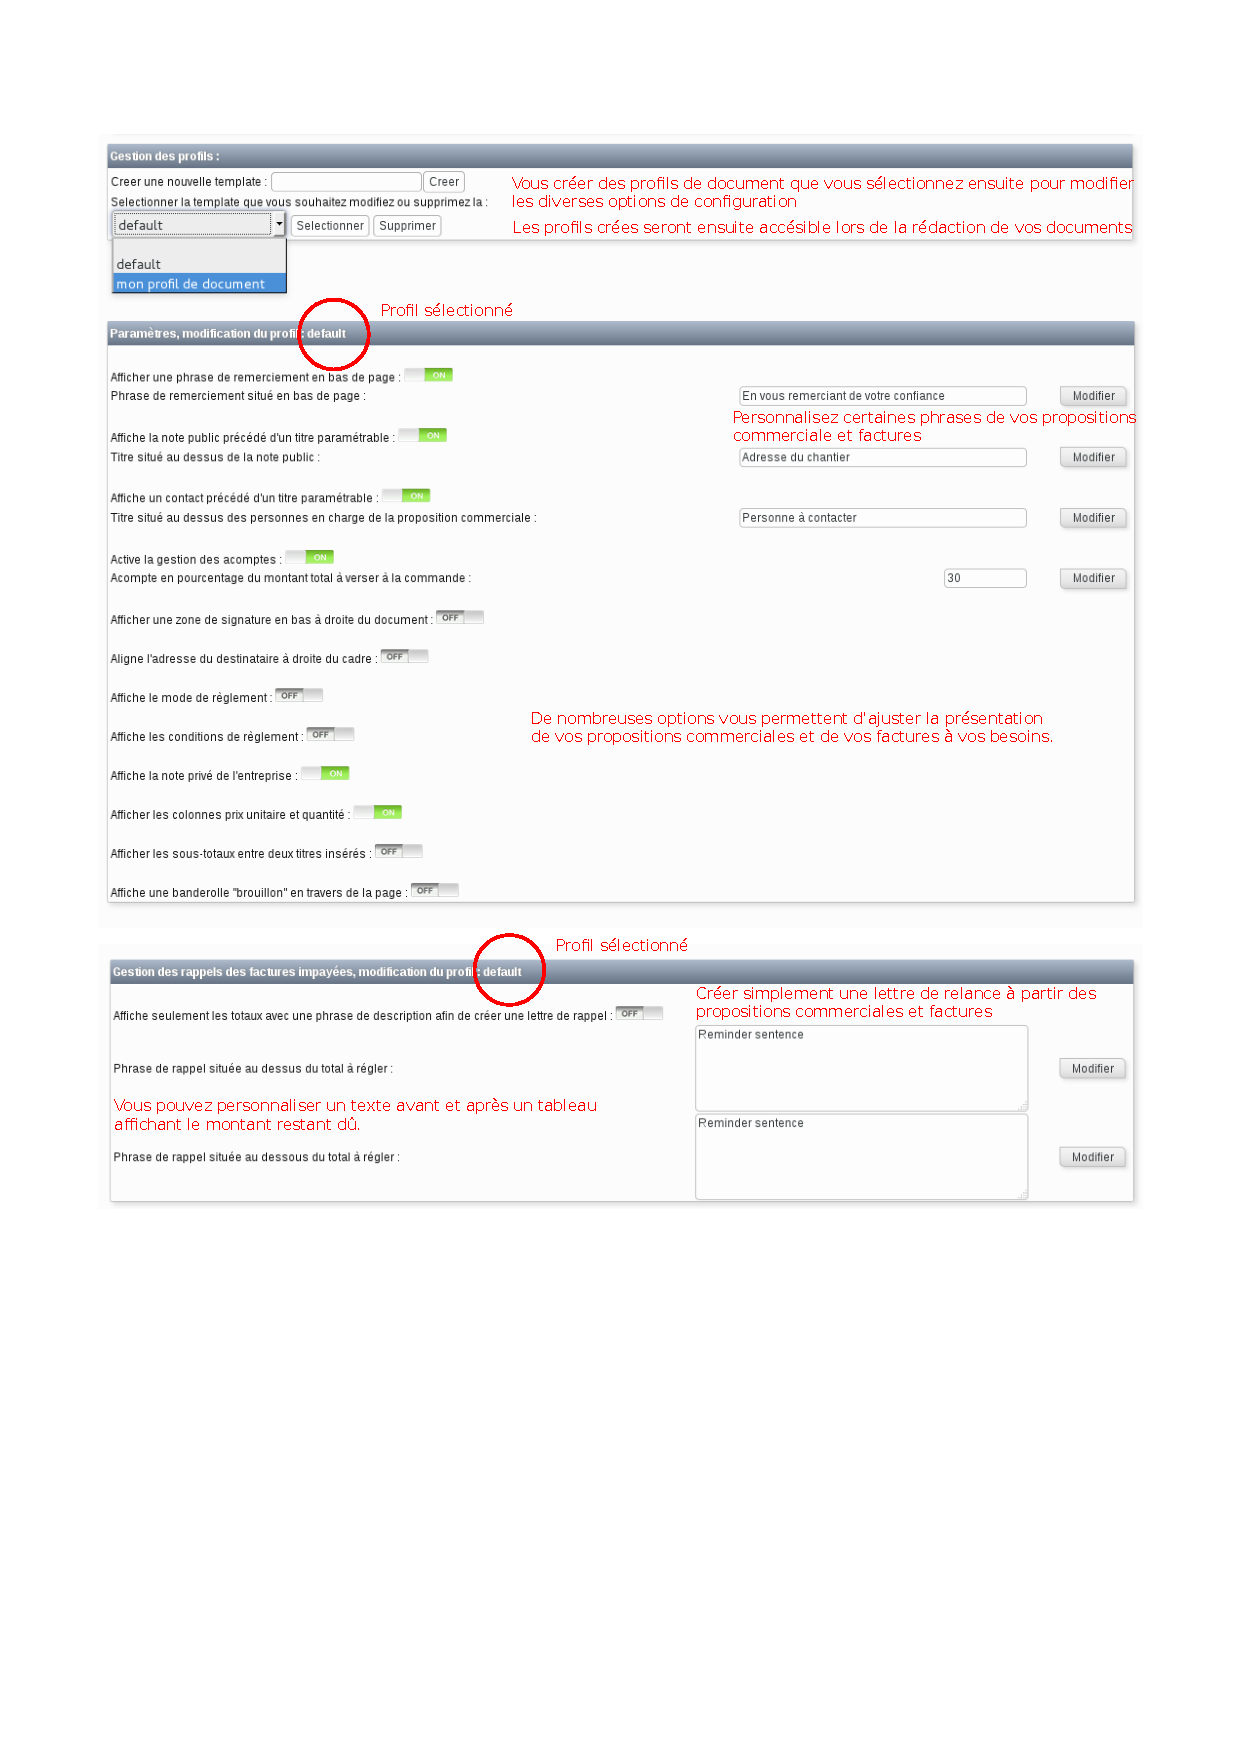
\includegraphics[height=25cm]{Configuration_annote.pdf}
  %  \caption{Organisation des interactions du programme avec les acteurs}
 %   \label{fig:Orga_logiciel}
 % \end{center}
%\end{figure}

%\begin{figure}
 % \begin{center}
   % \includegraphics[height=25cm]{Redaction_annote.pdf}
    %\caption{}
 %  \label{fig:Redact}
 % \end{center}
%\end{figure}


\end{document}
